\section{Dialogue Act Analysis}
    
    One way to view the structure of conversations is as a long string of adjacent dialogue acts (DAs).
    \subsection{Training Data}
        \subsubsection{SwDa}
        \subsubsection{MrDa}
    \subsection{Bi-LSTM-CRF \label{ssec: bi-lstm-crf}}
        \subsubsection{Initial Model}
        The model proposed in \cite{kumar2017dialogue} is a hierarchical Bi-LSTM-CRF model, which first encodes utterances using an embedding and LSTM layer and then uses these encoded utterances in a combination with another LSTM layer and a CRF layer to classify the dialogue acts of every utterance. The entire model is displayed in Fig. \ref{fig:kumar_model}.
        
        \begin{figure}[h]
            \centering
            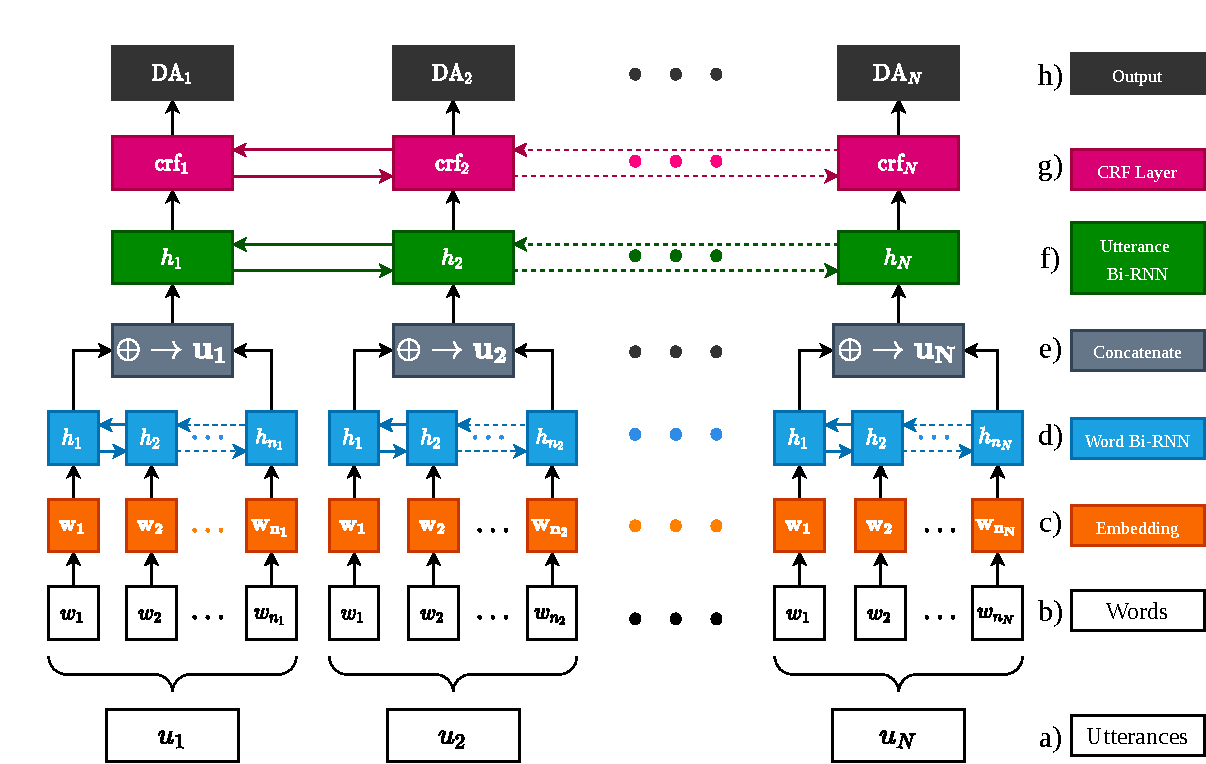
\includegraphics[width=\textwidth]{kumar.pdf}
            \caption{a) $N$ utterances $u_i$ are input into the model as b) a list of words $w_1 \dots w_{n_i}$. In c), the words are individually embedded into vectors $\mathbf{w_j}$ (see Sec. \ref{ssec: word embeddings}). The first Bi-RNN layer (on the word level), d), combines all $n_i$ words within $u_i$ into two vectors of numbers, one for the ``forward" direction and one for the ``backward" direction of the RNN (see Sec. \ref{ssec: bidirectional RNN}). In e), these vectors are concatenated into one vector $\mathbf{u_i}$ that can be understood as the embedding of the utterance $u_i$. In f), these utterance embeddings are again combined using a bi-directional RNN layer, but this time not just the two final states of the ``forward" and ``backward" direction are passed on, but all hidden states $h_i$ are (see Sec. \ref{ssec: outputting hidden states}). In g), a CRF layer makes the final classification, which is the sequence of dialogue acts $\text{DA}_i$ associated with utterances $u_i$ shown in h).}
            \label{fig:kumar_model}
        \end{figure}
        
        \subsubsection{New Implementation}
        \subsubsection{Memory Problems}
        \subsubsection{Improved Results}
        \subsubsection{Bi-GRU-CRF}